\documentclass[
    left=2.5cm,         % Sadly, generic margin parameter
    right=2.5cm,        % doesnt't work, as it is
    top=2.5cm,          % superseded by more specific
    bottom=3cm,         % left...bottom parameters.
    bindingoffset=6mm,  % Optional binding offset.
    nohyphenation=false % You may turn off hyphenation, if don't like.
]{eiti/eiti-thesis}
\langpol % Dla języka angielskiego mamy \langeng
\graphicspath{ {img/} }

\begin{document}

\EngineerThesis % Dla pracy inżynierskiej mamy \EngineerThesis
\instytut{Instytut Automatyki i Informatyki Stosowanej}
\kierunek{Informatyka}
\specjalnosc{Systemy Informacyjno-Decyzyjne}
\title
{
    Aplikacja do testowania odporności modeli klasyfikacyjnych \\
    na ataki z użyciem złośliwych danych \\
}

\engtitle
{ % Tytuł po angielsku do angielskiego streszczenia
    Unnecessarily long and complicated thesis' title \\
    difficult to read, understand and pronounce
}

\author{Jan Ambroziak}
\album{269260}
\promotor{dr inż. Paweł Zawistowski}
\date{\the\year}
\maketitle

%--------------------------------------
% Streszczenie po polsku
%--------------------------------------
\cleardoublepage % Zaczynamy od nieparzystej strony
\streszczenie \lipsum[1-3]
\slowakluczowe XXX, XXX, XXX

%--------------------------------------
% Streszczenie po angielsku
%--------------------------------------
\newpage
\abstract \kant[1-3]
\keywords XXX, XXX, XXX

%--------------------------------------
% Oświadczenie o autorstwie
%--------------------------------------
\cleardoublepage  % Zaczynamy od nieparzystej strony
\pagestyle{plain}
\makeauthorship

%--------------------------------------
% Spis treści
%--------------------------------------
\cleardoublepage % Zaczynamy od nieparzystej strony
\tableofcontents

%--------------------------------------
% Rozdziały
%--------------------------------------
\cleardoublepage % Zaczynamy od nieparzystej strony
\pagestyle{headings}

\section{Wstep}






Wraz z rozwojem i upowszechnianiem się modeli klasyfikujących obrazy graficzne,
pojawiają się nowe zagrożenia związane z bezpieczeństwem tej klasy rozwiązań.
Jednym z nich są złośliwe dane, które powodować mogą,
że pozornie dobrze działający klasyfikator zaczyna udzielać błędnych odpowiedzi.
Może to stanowić realne zagrożenie nawet dla życia i zdrowia ludzkiego
np. w przypadku gdy taki atak dotyczy systemu automatycznie sterującego pojazdem.

\subsection{Cel}
\label{sec:target}

Celem pracy inżynierskiej jest stworzenie aplikacji która ma wspierać testowanie
odporności modeli klasyfikacyjnych na ataki z użyciem złośliwych danych
Dla dostarczonego w narzuconej postaci modelu klasyfikatora możliwe będzie
przeprowadzenie ataku przy pomocy jednej z dostępnych metod.

\subsection{Istniejące rozwiązania}

Aktualnie na rynku znajduje się kilka rozwiązań implementujących podobne funkcjonalności
do tej która jest tu opisana. Warto zapoznać się z nimi oraz ich implementacjami.
Jednym z najbardziej populranych narzędzi tego typu jest \textit{CleverHans}\cite{DBLP:journals/corr/GoodfellowPM16}
wykorzystujący jako swoją bazę framework tensorflow oraz \textit{Adversarial Robustness Toolbox}\cite{DBLP:journals/corr/abs-1807-01069} opracowany przez IBM.
O ile \textit{CleverHans} z tytułu korzystania z tensorflow jest w stanie korzystać z akceleracji sprzętowej jaką zapewnia procesor graficzny, o tyle
\textit{Adversarial Robustness Toolbox} korzysta tylko i wyłącznie z mocy obliczeniowej głównego procesora.

\subsection{Użyte narzędzia}
Od czasu opublikowania przez firmę Google biblioteka Tensorflow \cite{DBLP:journals/corr/AbadiABBCCCDDDG16}
stała się jednym z wiodących narzędzi wykorzystywanych w branży. Prostota API i intuicyjność
języka Python, akceleracja obliczeń z wykorzystaniem procesorów graficznych oraz dobra integracja z
popularnymi bibliotekami dostępnymi dla języka Python czyni Tensorflow idealnym kandydatem.
W trakcie pracy wykorzystywałem głównie wysokopoziomowy interfejs Keras, który pozwala na szybkie
prototypowanie przez wysoki poziom abstrakcji jaki zapewnia. Keras zapewnia nam też dostęp do wytrenowanych modeli takich
InceptionV3\ref{InceptionV3} i MobileNetV2~\ref{MobileNetV2}, których wytrenowanie na potrzebę naszych testów byłoby
trudne z uwagi na ich złożoność.
Platforma testowa jakiej użyto to:
\begin{itemize}
    \item CPU: AMD Ryzen 3900X
    \item GPU: Nvidia GeForce 1060 GTX 6GB
    \item RAM: 32GB DDR4
    \item System Operacyjny: Windows 10
    \item Tensorflow wersja 2.2.0
    \item Interpreter Python 3.6.8 wersja 64bit
\end{itemize}
Wszystkie pozostałe biblioteki Python, wraz z wersjami, wykorzystane w projekcie, znajdują się w pliku
requirements.txt w folderze projektu.

\newpage
\section{Modele i dane testowe}
Aby sprawdzić poprawność implementacji oraz skuteczność ataków stworzono
kilka modeli klasyfikacyjnych o różnej złożoności, opartych o popularne zbiory danych
wykorzystywanych jako platforma testowa w publikacjach pokrewnych tematyką.

    \subsection{MNIST}
    Zbiór danych MNIST~\cite{mnist} to najprawdopodobniej najpopularniejszy zbiór związany z
    tematyką nauczania maszynowego.
    Zawiera on 60,000 obrazów o rozmiarach 28 na 28 pikseli, w skali szarości, przedstawiających
    odręcznie narysowane cyfry. Zbiór dzieli się na 50,000 przykładów używanych do
    trenowania modelu oraz 10.000 służących do testowania.
%        \subsubsection{Model Fully Connect}
%        Model FC to bardzo prosty model wykorzystujący tylko 4 warstwy perceptronów z sigmoidalną funkcja aktywacji
%        \todo{dodać obrazek}

        \subsubsection{Model Splotowy}
        Stworzony model splotowy to prosty przykład zastosowania splotowych sieci neuronowych, warstw Dropout i poolingu
        który w praktyce pozwala osiągnąć bardzo dobre wyniki dla zbioru MNIST. Tutaj posłużono sie przykładem ze
        Tensorflow Model Garden~\cite{tensorflow_model_garden} który jest stosunkowo prosty. Ta architektura pozwala nam
        na uzyskanie 93\% precyzji dla zbioru MNIST.
%        \todo{Dodać obrazek modelu}


        \subsubsection{LeNet5}
        LeNet5 to historycznie istotny model stworzony przez Yana LeCuna stworzony w latach 90tych
        jest jednym z najbardziej znanych zastosowań splotowych sieci neuronowych.
       \begin{figure}[H]
           \centring
            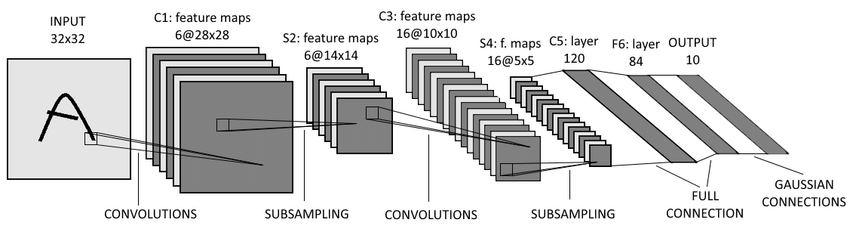
\includegraphics[width=\textwidth]{eiti/lenet5_overview.png}
            \caption{Struktura Modelu LeNet5\cite{LeNet5Diagram}}
       \end{figure}

    \subsection{CIFAR-10}
    Zbiór CIFAR-10 opisany w \textit{Learning Multiple Layers of Features from Tiny Images} \cite{Krizhevsky2009LearningML} zawiera kolorowe obrazy o rozdzielczości 32 na 32 piksele,
    podzielone na 10 klas takich jak np. koń, samolot czy żaba. Podobnie jak zbiór MNIST, CIFAR-10 zawiera
    60,000 obrazów podzielonych na 50,000 przykładów używanych do treningu jak i 10,000 do testowania.
    Aby usunąć problem nadmiernego dopasowania modeli obrazy z zbioru CIFAR10 używane
    do trenowania są losowo modyfikowane. Każdy obraz ma szanse 0.25
    na modyfikacje natężenia, nasycenia, kontrastu oraz odcienia. Dodatkowo każdy obraz może zostać obrócony bądź odbity.

%        \subsubsection{Model Splotowy CIFAR-10}
%        Tutaj w porównaniu do modelu dla zbioru MNIST wykorzystujemy także technikę normalizującą wartości wyjściowe
%        funkcji aktywacji (BatchNorm) w celu zwiększenia stabilności sieci (funkcja aktywacji ReLU nie posiada górnej granicy w
%        przeciwieństwie do funkcji sigmoidalnej). Poniżej znajduje się schemat zastosowanego modelu
        \subsubsection{SimpleNet CIFAR-10}
        Model SimpleNet opisany w
        \textit{Lets keep it simple, Using simple architectures to outperform deeper and more complex architectures}\cite{DBLP:journals/corr/HasanPourRVS16}
        jest odpowiedzią na bardziej złożone
        architektury sieci neuronowych (np. InceptionV3~\ref{InceptionV3}), które swoją nieznaczenie wyższą precyzję
        okupywały niewspółmiernie większą złożonością architektury i liczbą parametrów. SimpleNet wykorzystuje klasyczne
        techniki znane z splotowych sieci neuronowych takie jak batch normalization, warstwy splotowe, pooling,
        rektyfikująca funkcja aktywacji czy warstwy Dropout. Skutkiem tego jest model wymagający znacząco mniejszy nakładów
        obliczeniowych. Zarówno przy trenowaniu sieci jak i przy klasyfikacji. Model WRN\cite{DBLP:journals/corr/ZagoruykoK16}
        posiadający 11 milionów parametrów uzyskuje precyzję na poziomie około 95\% dla zbioru CIFAR-10.
        SimpleNet uzyskuje w naszej implementacji precyzję 91.4\% dla około 5 milionów parametrów.
        Autorzy SimpleNet zgłaszał precyzję modelu na poziomie 95.51\% natomiast precyzja na poziomie 91.4\% jest wystarczająca do naszych potrzeb.
        Z uwagi na to że nie jest dostępna oficjalna wersja modelu SimpleNet kompatybilna z tensorflow, konieczne było stworzenie własnej.
        Zaimplementowana wersja modelu uzyskuje precyzję dla zbioru CIFAR-10 porównywalną z tą którą zaprezentowali autorzy.
        \begin{figure}[H]
            \centring
            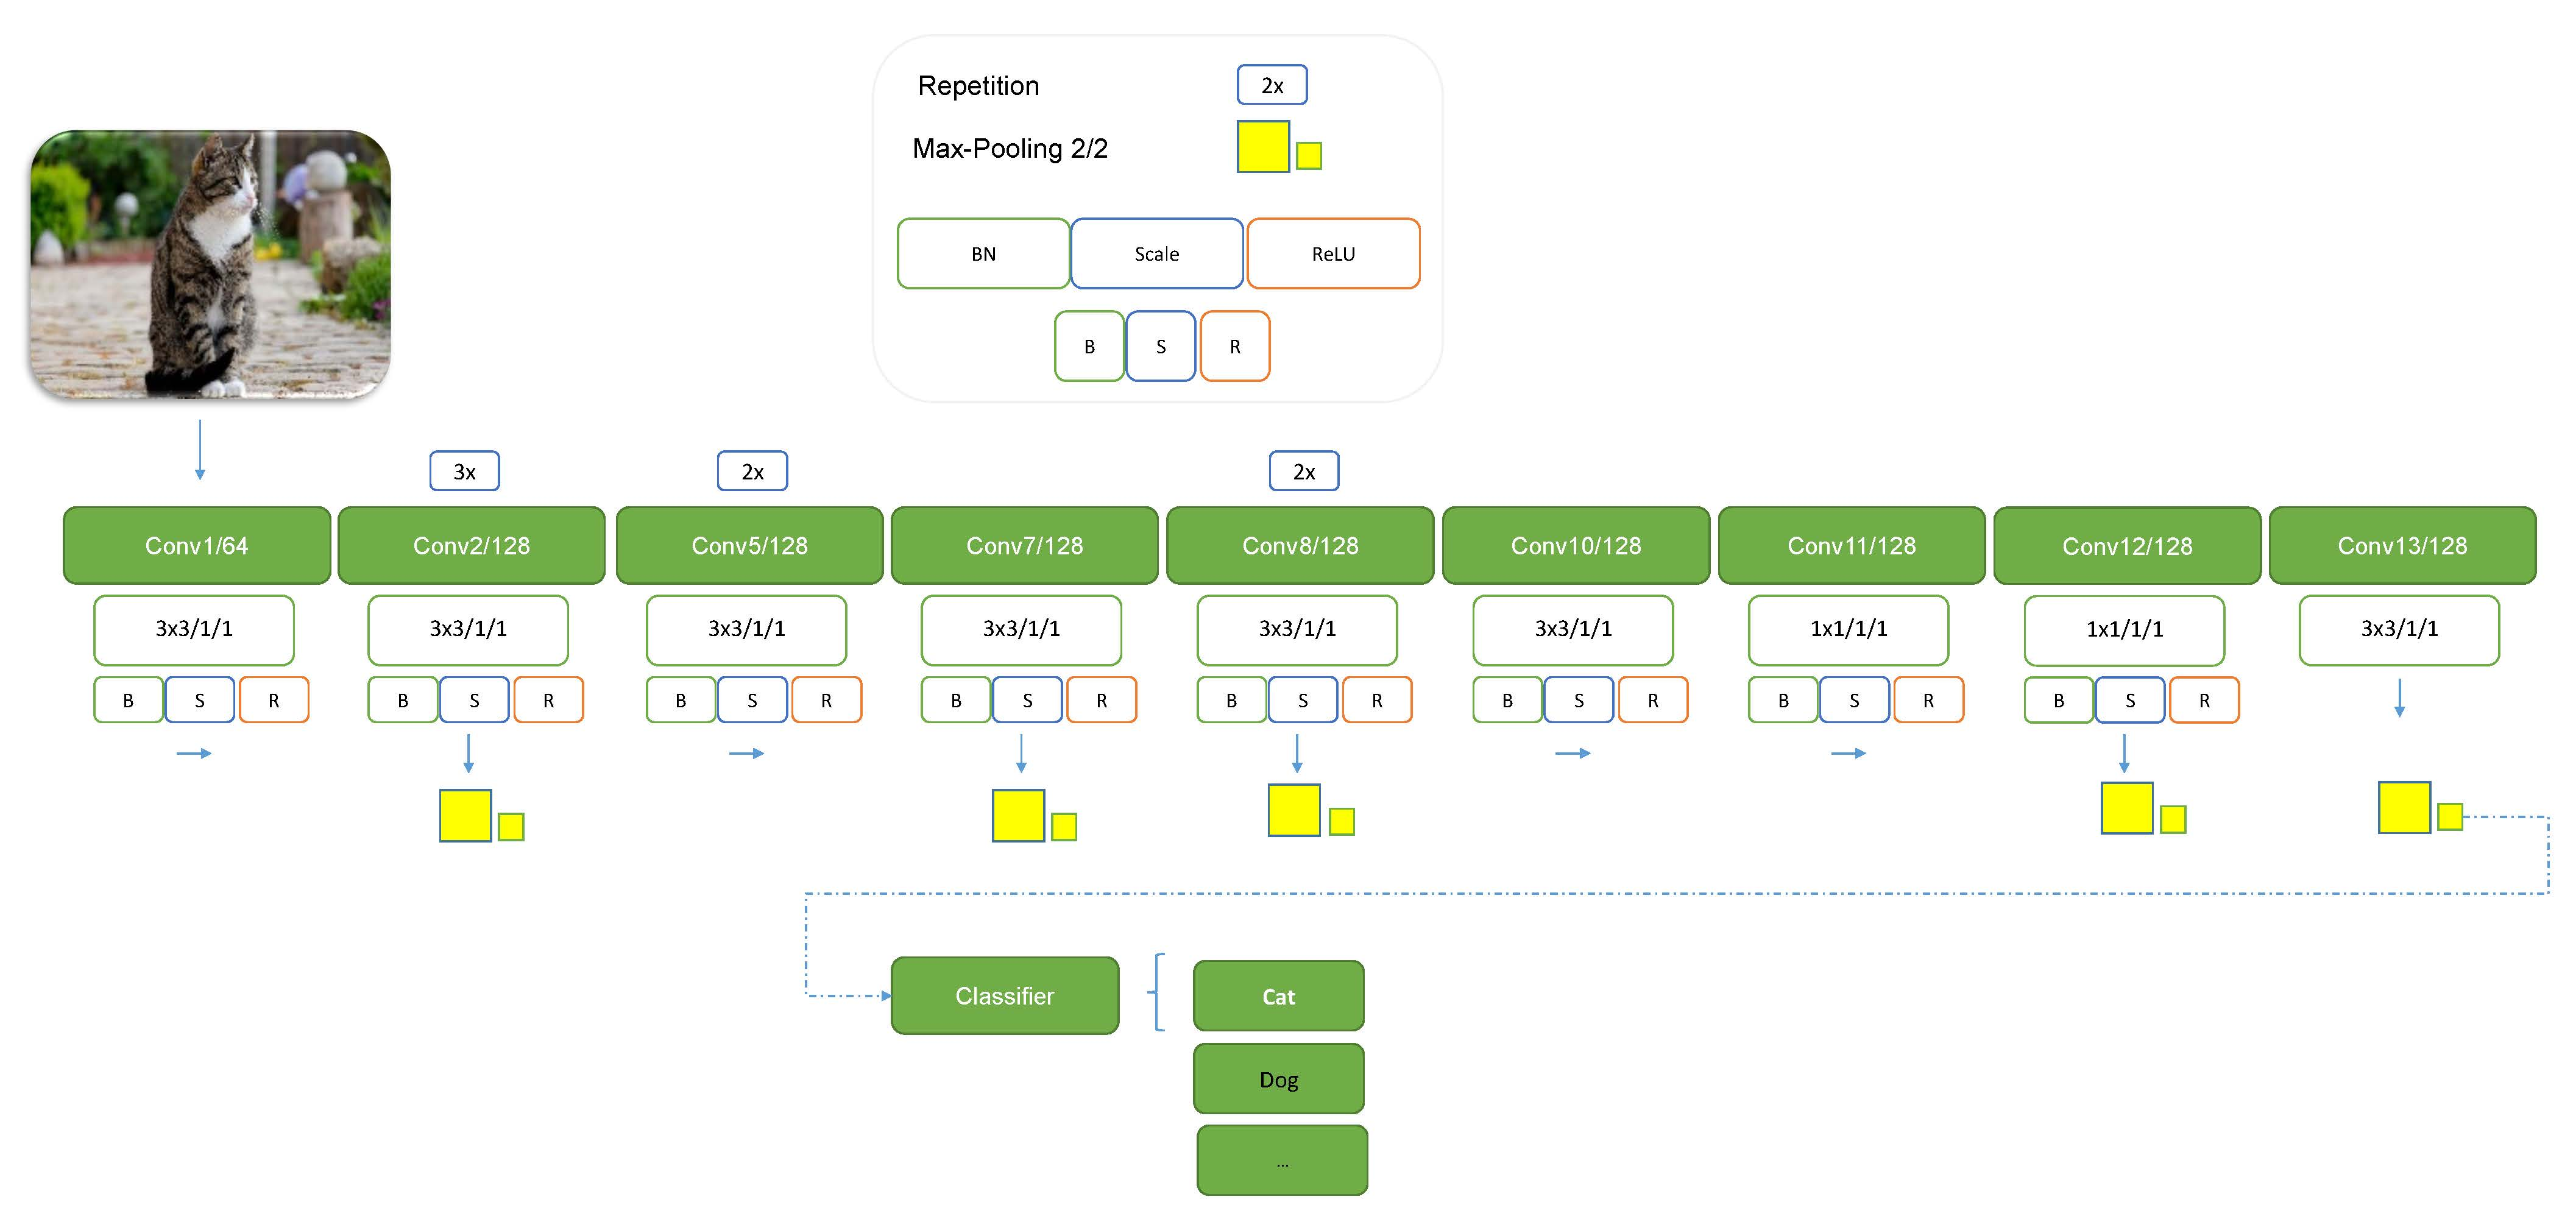
\includegraphics[width=\textwidth]{eiti/simplenet_overview.jpg}
            \caption{Schemat modelu SimpleNet}
        \end{figure}

    \subsection{CIFAR-100}
    Zbiór CIFAR100 opisany, podobnie jak CIFAR-10 w  \textit{Learning Multiple Layers of Features from Tiny Images} \cite{Krizhevsky2009LearningML}
    jest zbiorem obrazów, o rozdzielczości 32x32 pikseli z trzema kanałami kolorów, podzielonym na 100 klas.
    Każda klasa posiada w tym zbiorze 600 przykładów, z czego 500 jest przykładami treningowymi, a 100 przykładami testowymi.
        \subsection{SimpleNet CIFAR-100}
        Jako klasyfikator dla zbioru CIFAR-100 wybrany został także model SimpleNet. Architektura sieci i sposób trenowania
        jest identyczny jak w przypadku zbioru CIFAR-10. Jedyną różnicą jest zbiór treningowy którym w tym przypadku jest CIFAR-100.
        Autorzy modelu~\cite{DBLP:journals/corr/HasanPourRVS16} zgłaszają dla zbioru CIFAR-100 precyzję top-1 na poziomie 73.42\%.
        Nasza implementacja uzyskuje precyzję top-1 na poziomie 70.73\% i top-5 na poziomie 92.21\%

%        \subsubsection{Model Splotowy CIFAR-100}
%        Model którego używamy do klasyfikacji obrazów jest analogiczny do modelu użytego w przypadku zbioru CIFAR-10 z jedyną różnicą polegającą na
%        tym że filtry splotowe posiadają większe wymiary. Poniżej znajduje się schemat zastosowanego modelu

    \subsection{ILSVRC2012}\label{ILSVRC2012}
        Zbiór ILSVRC 2012 popularnie nazywany zbiorem ImageNet to, bazowany na bazie danych obrazów ImageNet, zbiór
        przygotowany specjalnie pod konkurs\textit{ImageNet Large Scale Visual Recognition Challenge} \cite{ILSVRC15}.
        Baza danych ImageNet bazuje na bazie WordNet i tworzy hierarchie obrazów uporządkowaną względem synsetów
        czyli zbiorów synonimów (syn od synonim i set z ang. zbiór). Zbiór ILSVRC 2012 posiada 1000 klas i około 1000
        obrazów dla każdej klasy. Obrazy mają rozdzielczośc 299x299 pikseli oraz 3 kanały kolorów. Łącznie zbiór posiada
        1281167 przykładów treningowych oraz 50000 przykładów testowych.

        \subsubsection{InceptionV3}\label{InceptionV3}
            InceptionV3 to zaproponowany przez autorów
            \textit{Rethinking the Inception Architecture for Computer Vision}\cite{DBLP:journals/corr/SzegedyVISW15}
            model którego celem było umożliwienie skalowania architektur modeli splotowych przy ograniczeniu wzrostu
            wymaganej mocy obliczeniowej za pomocą zastosowania warstw "Inception".
            InceptionV3 uzyskuje precyzje top-1 na poziomie 78.8\% oraz precyzję top-5 na
            poziomie 94.4\% dla zbioru ILSVRC~\ref{ILSVRC2012} w implementacji dostarczanej przez bibliotekę Keras.
            Jest to też największy z wykorzystanych modeli. Posiada ponad 23 miliony parametrów oraz 159 warstw.
            \begin{figure}[H]
            \centring
            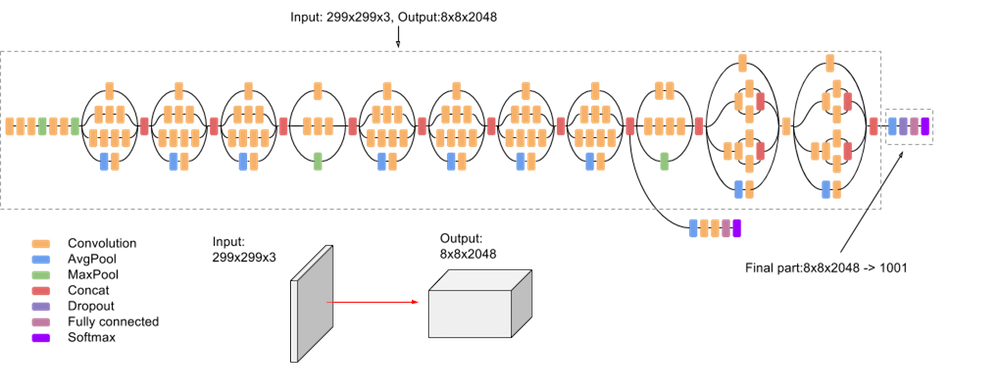
\includegraphics[width=\textwidth]{eiti/inceptionv3overview.png}
            \caption{Schemat modelu InceptionV3}
            \end{figure}

%        \subsubsection{ResNetV2}
%            Autorzy \textit{Identity Mappings in Deep Residual Networks}\cite{DBLP:journals/corr/HeZR016}
%            zaproponowali model należący do grupy modeli nazywanych głębokimi sieciami rezydualnymi (z ang. Deep Residual Networks)
%            nazwany ResNetV2. Jeden z najbardziej złożonych wariantów modelu ResNetV2 - ResNet152
%            uzyskuje precyzję top-1 na poziomie 78.7\% i top-5 94.5\% dla zbioru ILSVRC2012.\ref{ILSVRC2012}.
%            W trakcie pracy, z uwagi na mniejsze wymogi obliczeniowe , użyty został model ResNet50v2, który jest
%            nieco zmniejszoną wersją oryginalnego modelu. Uzyskuje on precyzję top-1 na poziomie 74.9\% i top-5 92.1\%.
%            \begin{figure}[H]
%            \centring
%            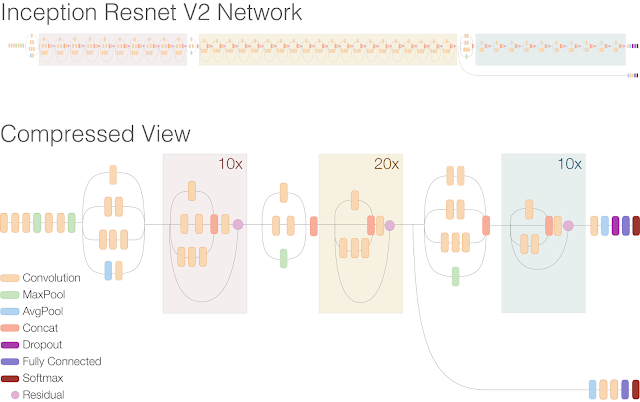
\includegraphics[width=\textwidth]{eiti/resnetv2overview.png}
%            \caption{Schemat modelu ResNetV2}
%            \end{figure}

        \subsubsection{MobileNetV2}\label{MobileNetV2}
            Autorzy \textit{Inverted Residuals and Linear Bottlenecks: Mobile Networks for Classification}\cite{DBLP:journals/corr/abs-1801-04381}
            stworzyli model którego celem, podobnie jak SimpleNet, było zmniejszenie rozmiarów sieci i potrzebnych nakładów obliczeniowych
            do jej używania, przy jednoczesnym zachowaniu wysokiego poziomu precyzji. W tym celu autorzy wykorzystali
            zmodyfikowaną wersję warstw rezydualnych (z ang. residual layer) z takich modeli jak np. ResNet\cite{DBLP:journals/corr/HeZR016}.
            O ile autorzy modelu SimpleNet, starał się uzyskać
            podobny cel dla zbiorów CIFAR-10 i CIFAR-100, tak tutaj autorzy skupili się przede wszystkim na zbiorze ILSVRC.
            MobileNetV2 działa z precyzją top-1 na poziomie 70.6\% i top-5 89.8\% w implementacji dostarczanej przez bibliotekę Keras.
            MobileNetV2 posiada 4.2 miliona parametrów oraz 88 warstw.

            \begin{figure}[H]
            \begin{center}
            \caption{Schemat warstwy \textit{residual bottleneck}}
            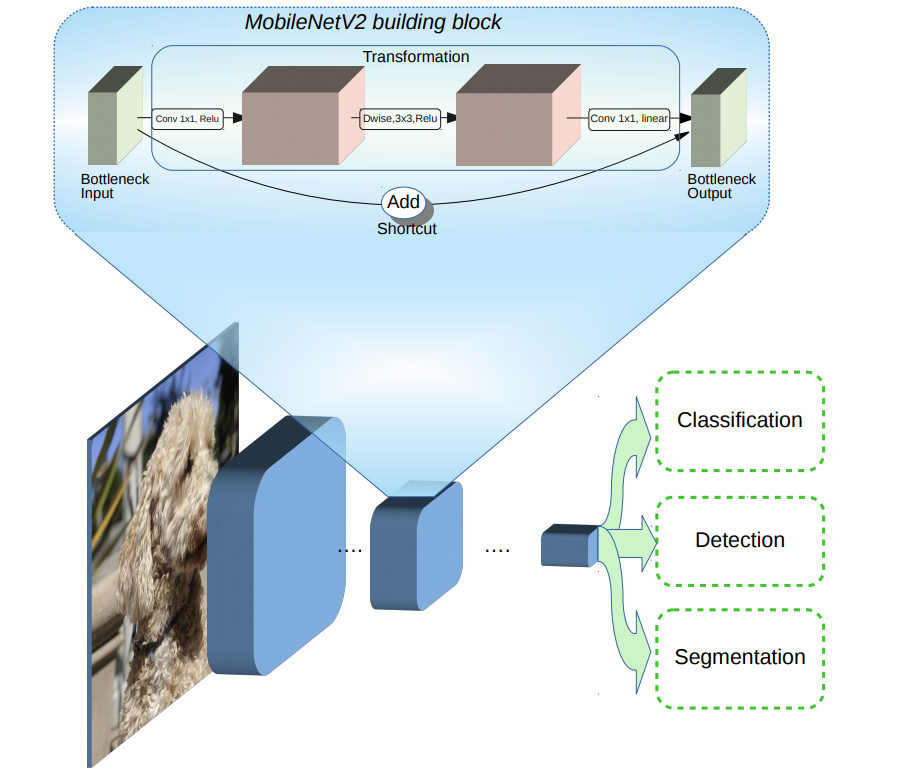
\includegraphics[width=0.6\textwidth]{eiti/mobilenetv2_overview.png}
            \end{center}
            \end{figure}

            \begin{table}[H]
            \centering
            \caption{Tabela z warstwami wykorzystanymi w sieci MobileNetV2}
            \begin{array}{c|c|c|c|c|c}
                \text { Input } & \text { Operator } & t & c & n & s \\
                \hline 224^{2} \times 3 & \text { conv2d } & - & 32 & 1 & 2 \\
                112^{2} \times 32 & \text { bottleneck } & 1 & 16 & 1 & 1 \\
                112^{2} \times 16 & \text { bottleneck } & 6 & 24 & 2 & 2 \\
                56^{2} \times 24 & \text { bottleneck } & 6 & 32 & 3 & 2 \\
                28^{2} \times 32 & \text { bottleneck } & 6 & 64 & 4 & 2 \\
                14^{2} \times 64 & \text { bottleneck } & 6 & 96 & 3 & 1 \\
                14^{2} \times 96 & \text { bottleneck } & 6 & 160 & 3 & 2 \\
                7^{2} \times 160 & \text { bottleneck } & 6 & 320 & 1 & 1 \\
                7^{2} \times 320 & \text { conv2d 1x1 } & - & 1280 & 1 & 1 \\
                7^{2} \times 1280 & \text { avgpool 7x7 } & - & - & 1 & - \\
                1 \times 1 \times 1280 & \text { conv2d 1x1 } & - & \mathrm{k} & - & \\
                \hline
            \end{array}
            \end{table}

\begin{table}[ht]
\centering
\caption{Precyzja top-1 i top-5 wykorzystywanych przez nas modeli}
\begin{adjustbox}{max width=\textwidth}
\begin{pycode}
from latex_utils import *
generate_accuracy_table_for_all()
\end{pycode}
\end{adjustbox}
\end{table}


\newpage
\section{Rodzaje Ataków}
Ideą ataków adwersaryjnych
%\todo{tu dodać definicje} jest osiągnięcie jednego z wymienionych celów:
\begin{enumerate}
    \item Zmniejszenie prawdopodobieństwa z jakim model klasyfikuje przykład
    \item Zła klasyfikacja przykładu wejściowego (niezaleznie od końcowej klasy)
    \item Przyporządkowanie przykładu wejściowego do złej, zadanej z góry klasy
%    \todo{Sprawdzić i dodać cytowanie}
\end{enumerate}

Możemy też rozróżnić ataki z uwagi na to jakie dane są dostępne dla algorytmu atakującego:
\begin{enumerate}
    \item Dostępny jest gradient, funkcja kosztu i funkcja trenująca
    \item Dostępna jest tylko funkcja kosztu
    \item Dostępny jest przykład
    \item Dostępne są tylko dane wejściowe i klasa do jakiej model przyporządkowuje dany przykład
%    \todo{poprawić powyższe i dodać cytowanie}

\end{enumerate}

\newpage
\section{Wykorzystane Ataki}
W projekcie zaimplementowanych zostało kilka ataków które zostały opisane w anglojęzycznych publikacjach.
Poniżej znajdują się ich opisy, uwagi dotyczące implementacji, przykłady zastosowania oraz wyniki testów
zastosowanych do oceny ataków. Szersza dyskusja dotycząca użyteczności oraz porównanie znajdują się w sekcji \ref{comparison}

\subsection{FGSM}
    FGSM czyli Metoda szybkiego znaku gradientu (z ang. Fast Gradient Sign Method) opsiana w artykule
    pod tytułem \textit{Explaining and Harnessing Adversarial Examples}\cite{harnessing} to jedna z pierwszych
    opisanych metod ataku na modele klasyfikacyjne wykorzystujący złośliwe dane.
    Aby wygenerować złośliwy przykład metoda ta wymaga znajomości gradientu funkcji kosztu obliczanego względem danych
    wejściowych oznaczonego jako

    \begin{equation}
        \nabla_{x} J(x, y).
        \qquad\text{gdzie}
        \begin{tabular}[t]{ll}
        $x$   & -- dane wejściowe \\
        $y_{prawdziwe}$   & -- klasa do której należą dane wejściowe\\
        $J(x, y_{prawdziwe})$  & -- funkcja kosztu \\
        $\nabla_{x}$  & -- gradient względem danych wejściowych \\
        \end{tabular}
    \end{equation}

    Idea metody polega na dodaniu bądź odjęciu małej, arbitralnie ustalonej, wartości (oznaczanej przez \(\epsilon\)) do
    danych wejściowych w zależności od znaku gradientu tak aby zwiększyć wartość funkcji kosztu,
    doprowadzając do niepoprawnej klasyfikacji danych wejściowych zmodyfikowanych w niewielkim stopniu.
    Możemy zapisać to działanie w następujący sposób.

    \begin{equation}
    x' = x + \epsilon\operatorname{sign}(\nabla_{x} J(x, y_{prawdziwe}))
    \qquad\text{gdzie}
    \begin{tabular}[t]{ll}
    $x'$  & -- spreparowany przykład ze złośliwymi danymi \\
    \end{tabular}
    \end{equation}

    Analogiczny przykład do tego znajdującego się w oryginalnej publikacji\cite{harnessing} znajduje się poniżej.
%    \todo{tutaj wstawić przykład z dodawaniem obrazków}

    Podstawową wadą opisywanej metody jest fakt że nie mamy wpływu na to jaka będzie klasa wyjściowa
    spreparowanych przez nas danych wejściowych. Kolejną jest to że niektóre dane i modele wymagają od nas
    doboru wysokiej wartości parametru $\epsilon$ aby być w stanie spreparować pożądane dane, co z kolei powoduje dużą
    różnicę między danymi wejściowymi a tymi utworzonymi w toku stosowania metody.
    W publikacji pod tytułem \textit{Adversarial examples in the physical world}\cite{DBLP:journals/corr/KurakinGB16}
    autorzy opisują kilka metod pochodnych do FGSM.

    \subsubsection{I-FGSM}
    I-FGSM czyli Iteracyjna Metoda Szybkiego Znaku Gradientu (z ang. Iterative Fast Gradient Sign Method) to metoda
    które rozwiązuje problem konieczności doboru wysokiej wartości $\epsilon$ poprzez zastosowanie metody FGSM kilkakrotnie
    ,jednocześnie zapewniając pod koniec każdego kroku że przyogotowany każdy piksel obrazu nie różni się od oryginału o więcej
    niż $\epsilon$, z niższą wartością parametru $\epsilon$ niż wymagane oryginalnie w metodzie jednokrokowej.
    Pozwala to  potencjalnie ogarniczyć różnicę między preparowanymi przez nas danymi a oryginalnymi danymi wejściowymi
    oraz przerwanie działania metody kiedy model przestania poprawnie klasyfikować dane wejściowe.

    \begin{algorithm}
    \caption{I-FGSM}\label{IFGSM}
    \begin{algorithmic}[1]
    \State $i \gets 0$
    \While{$i <  i_{max}$}
        \State $x' = x + \alpha\operatorname{sign}(\nabla_{x} J(x, y_{prawdziwe}))$
        \State $i \gets i+1$
        \State $Przytnij(x', \epsilon)$
    \EndWhile
    \end{algorithmic}
    \end{algorithm}

    \subsubsection{LL-FGSM}
    LL-FGSM (z ang. Least Likely FGSM) to metoda pozwalająca nam na spreparowanie danych które będę przydzielane do
    konkretnej klasy (ozn. $y_{celu}$), a nie tylko na niepoprawną klasyfikacje. W tym wypadku zamiast starać się
    zmieniać wartości pikseli obrazu zgodnie z kierunkiem gradientu funkcji kosztu dla prawidłowej klasy
    staramy się zmieniać wartości pikseli przeciwnie do kierunku gradientu funkcji kosztu dla klasy $y_{celu}$.
    Intuicyjnie można to opisać jako nie oddalanie się od prawdziwej klasy obrazu, a jako przybliżanie się do zadanej
    przez nas klasy.
    Autorzy metody zwracają uwagę na przydatność tej metody
    w przypadku gdy korzystamy z modeli operujących wieloma klasami i gdzie różnice między obiektami z różnych klas mogą
    być bardzo niewielkie (np. między rasami psów). Metoda ta jest także iteracyjna i zapewnie różnice między
    odpowiednimi pikselami obrazów nie większą niż $\epsilon$ więc można uznać ją za rozszerzenie metody I-FGSM.

    \begin{algorithm}
    \caption{LL-FGSM}\label{LLFGSM}
    \begin{algorithmic}[1]
    \State $i \gets 0$
    \While{$i <  i_{max}$}
        \State $x' = x - \alpha\operatorname{sign}(\nabla_{x} J(x, y_{celu}))$
        \State $i \gets i+1$
        \State $Przytnij(x', \epsilon)$
    \EndWhile
    \end{algorithmic}
    \end{algorithm}


\subsection{DeepFool}
W publikacji \textit{DeepFool: a simple and accurate method to fool deep neural networks}\cite{DBLP:journals/corr/Moosavi-Dezfooli15}
autorzy proponują metodę alternatywną do FGSM mającą minimalizować wprowadzaną do danych wejściowych perturbacje jednocześnie
osiągając zmianę klasy do której model przyporządkowuje dane wejściowe.
%Punktem wyjściowym rozważań autorów było założenie
%że model z którego korzystamy jest przekształceniem afinicznym, opracowanie metody pozwalającej na
%uzyskanie zminimalizowanej perturbacji, a następnie zgeneralizowanie metody dla modeli nie będących przekształceniami afinicznymi.
Wadą DeepFool jest brak możliwości narzucenia klasy do której chcielibyśmy aby przyporządkowywane były nasze zmodyfikowane dane.
Metoda ta jest nieco bardziej złożona obliczeniowo jako że pojedynczy krok algorytmu wymaga od nas obliczenia gradientu dla
prawdopodobieństwa każdej klasy względem danych wejściowych, co przy zbiorach danych z wieloma klasami
takich jak np. ImageNet może być problematyczne. Poniżej znajduje się pseudokod opisujący metodę DeepFool dla modelu
wieloklasowego.
\begin{algorithm}
\caption{DeepFool}\label{DeepFool}
\begin{algorithmic}[1]
\State $x_0 \gets x$
\While{$f(x_{i}) =  y_{prawdziwe}$}
\For{$k \neq \hat{k}(x_{0})$}
    \State $w'_k\gets \nabla f_k(x_i) - \nabla f_{\hat{k}(x_0)}(x_i)$
    \State $f'_k\gets f_{k}(x_i) - f_{\hat{k}(x_0)}(x_i)$
\EndFor
\State $\hat{l}\gets \arg \min_{k\neq\hat{k}(x_0)} \dfrac{|f'_k|}{||w'_k||_2}$
\State $r_i\gets \dfrac{|f'_{\hat{l}}|}{||w'_{\hat{l}}||^2_2}w'_{\hat{l}}$
\State $x_{i+1}\gets x_i + r_i$
\State $i\gets i + 1$
\EndWhile
\State \textbf{return} $\hat{r} = \sum_{i} r_i$
\end{algorithmic}
\end{algorithm}




\subsection{L-BFGS-B}
Metoda opisana w \textit{Intriguing properties of neural networks}\cite{DBLP:journals/corr/SzegedyZSBEGF13}
to próba rozwiązania poniższego problemu optymalizacyjnego w celu uzyskania minimalnej perturbacji danych wejściowych
która powoduje niepoprawną klasyfikacje danych przez model:
    \begin{equation}
    \min{\| r\|_{2}}
    \qquad\text{przy warunkach:}
    \begin{tabular}[t]{ll}
    f(x + r) = $y_{celu}$ \\
    $x+r \in [0,1]^{m}$ \\
    \end{tabular}
    \qquad\text{gdzie:}
    \begin{tabular}[t]{ll}
    r - perturbacja \\
    \end{tabular}
    \end{equation}
Znalezienie dokładnego rozwiązania powyższego problemu jest skomplikowane, dlatego autorzy postanowili szukać aproksymacji
rozwiązania poprzez liniowe przeszukiwanie w celu znalezienia najmniejszej wartości parametru $c > 0$ dla którego spełniony
zostaje warunek $f(x+r) = y_{celu}$ gdzie $r$ uzyskujemy z zastosowania algorytmu L-BFGS-B dla poniższego problemu:
    \begin{equation}
    \min{c| r| + J(x+r, y_{celu})}
    \qquad\text{przy warunkach:}
    \begin{tabular}[t]{ll}
    $x+r \in [0,1]^{m}$ \\
    \end{tabular}
    \end{equation}



\subsection{JSMA}
Idea ataku JSMA (Jacobian Saliency Map Attack) opisanego w
\textit{The Limitations of Deep Learning in Adversarial Settings}\cite{DBLP:journals/corr/PapernotMJFCS15}
polega na utworzeniu mapy istotności (z ang. Saliency Map) pikseli obrazu dla każdej z klas.
Dzięki temu jesteśmy w stanie określić jak dane piksele w obrazie wpływają na określanie prawdopodobieństwa należenia
do danej klasy przez model. Sposób tworzenia mapy istotności jest zamieszczony poniżej:
\begin{equation}\label{jsma+}
S^{+} ( \mathbf { x } , y ) [ i ] = \left\{ \begin{array} { c } { 0 \text { jeśli } \frac { \partial \mathbf {f} _ { y } ( \mathbf {x} ) } { \partial \mathbf {x} _ { i } } < 0 \text { lub } \sum _ { j \neq y } \frac { \partial \mathbf {f} _ { j } ( \mathbf {x} ) } { \partial \mathbf {x} _ { i } } > 0 } \\ { \left( \frac { \partial \mathbf {f} _ { y } ( \mathbf {x} ) } { \partial \mathbf {x} _ { i } } \right) \left| \sum _ { j \neq y } \frac { \partial \mathbf {f} _ { j } ( \mathbf {x} ) } { \partial \mathbf {x} _ { i } } \right| \text { w.p.p } } \end{array} \right.
\qquad\text{gdzie:}
\begin{tabular}[t]{ll}
x - dane wejściowe \\
${f} _ { y } ({x})$ - prawd. przynależności x do klasy y \\
$x_{i}$ - i-ty piksel obrazu wejściowego x \\
S({x},y)[i] - wartość i-tego piksel dla klasy y
\end{tabular}
\end{equation}

W powyżej zdefiniowanej mapie nieujemne wartości oznaczają poziom wpływu zwiększenia intensywności danego piksela $i$
na przynależność dla danej klasy $y$.
Warunek $\frac { \partial \mathbf {f} _ { y } ( \mathbf {x} ) } { \partial \mathbf {x} _ { i } } < 0$
zapewnia że nie będziemy rozpatrywać pikseli które mają negatywny wpływ na wartość prawdopodobieństwa należenia przykładu
do klasy $y$.
Natomiast warunek $\sum _ { j \neq y } \frac { \partial \mathbf {f} _ { j } ( \mathbf {x} ) } { \partial \mathbf {x} _ { i } } > 0 $
zapewnia że nie będziemy rozpatrywać pikseli które mają pozytywny wpływ na wartość prawdopodobieństwa należenia przykłady do klas
innych niż narzucona przez nas klasa $y$. Autorzy metody proponują też analogiczną mapę istotności w która
zamiast określać wpływ zwiększenia intensywności pikseli na przynależność przykładu do danej klasy określa wpływ zmniejszania
intensywności piksela na przynależność do danej klasy.

%\begin{equation}\label{jsma-}
%S^{-} ( \mathbf { x } , y ) [ i ] = \left\{ \begin{array} { c } { 0 \text { jeśli } \frac { \partial \mathbf {f} _ { y } ( \mathbf {x} ) } { \partial \mathbf {x} _ { i } } > 0 \text { lub } \sum _ { j \neq y } \frac { \partial \mathbf {f} _ { j } ( \mathbf {x} ) } { \partial \mathbf {x} _ { i } } < 0 } \\ { \left|( \frac { \partial \mathbf {f} _ { y } ( \mathbf {x} ) } { \partial \mathbf {x} _ { i } } )\right  \left| \sum _ { j \neq y } \frac { \partial \mathbf {f} _ { j } ( \mathbf {x} ) } { \partial \mathbf {x} _ { i } } \right \text { w.p.p } } \end{array} \right.
%\end{equation}

W praktyce jednak większość pikseli nie spełnia warunków określonych w pierwszej linii podanych równań,
dlatego autorzy zastosowali metodę wyboru par pikseli $p_1$ i $p_2$ zamiast pojedynczego piksela.
W tym celu stosowana jest opisana poniżej metoda.

\begin{equation} \label{saliency_map}
\arg \max _ { \left( p _ { 1 } , p _ { 2 } \right) } \left( \sum _ { i = p _ { 1 } , p _ { 2 } } \frac { \partial \mathbf { f } _ { y } ( \mathbf { x } ) } { \partial \mathbf { x } _ { i } } \right) \times \left| \sum _ { i = p _ { 1 } , p _ { 2 } } \sum _ { j \neq y } \frac { \partial \mathbf { f } _ { j } ( \mathbf { x } ) } { \partial \mathbf { x } _ { i } } \right|
\end{equation}

O ile rozwiązuje to problem znalezienia pikseli które spełniają warunki o tyle metoda ta ma większą złożoność obliczeniową
z uwagi na to że musimy rozpatrzyć wszystkie możliwe pary pikseli zamiast tylko pojedynczych pikseli.
Opisany poniżej algorytm oddaje istotę opisanej przez autorów metody.

\begin{algorithm}
\caption{JSMA}\label{JSMA}
\begin{algorithmic}[1]
\State $x' \gets x$
\While{$f(x') \neq  y_{celu}\ \& \ i < i_{max}$}
    \State $p_1, p_2$ = S$(x',y_{celu})$ \Comment przez S rozumiemy (\ref{saliency_map})
    \State zmodyfikuj $p_1$ i $p_2$ o $\theta$
    \State jeśli $p_1$ lub $p_2$ wynosi 0 albo 1 usuń je z listy pikseli
    \State $i \gets i+1$
\EndWhile
\State \textbf{return} $x'$
\end{algorithmic}
\end{algorithm}

Istnieje wiele różnych wariantów metody JSMA, których zasadnicze działanie nie różni się bardzo od tego opisanego powyżej.
\textit{Maximal Jacobian-based Saliency Map Attack}\cite{DBLP:journals/corr/abs-1808-07945} przeprowadza bardzo
zwięzłe podsumowanie różnych wariantów metody JSMA. Warto tutaj przytoczyć kilka różnic między opisanymi w tej publikacji
wariantami JSMA.

\subsubsection{JSMA+ i JSMA-}
Autorzy \textit{Maximal Jacobian-based Saliency Map Attack}\cite{DBLP:journals/corr/abs-1808-07945} wprowadzają rozróżnienie
pomiędzy JSMA+ a JSMA- w zależności od tego czy intensywność pikseli jest zmniejszana i wykorzystywane są warunki~(\ref{jsma-})
czy też intensywność pikseli jest zwiększana i wykorzystywane są warunki~(\ref{jsma+})

\subsubsection{JSMA-F i JSMA-Z}
W publikacji \textit{Towards Evaluating the Robustness of Neural Networks}\cite{DBLP:journals/corr/CarliniW16a}
autorzy proponują rozróżnienie pomiędzy JSMA-F, które w metodzie~(\ref{saliency_map}) wykorzystuje do obliczania pochodnej cząstkowej
wyjście funkcji softmax stosowanej zazwyczaj jako ostatnia warstwa modelu, a JSMA-Z które zamiast tego wykorzystuje wektor
wyjściowy przedostatniej warstwy określany często jako zazwyczaj jako logits.

\subsubsection{NT-JSMA}
NT-JSMA czyli wersja JSMA bez zadanej klasy którą chcemy osiągnąć (z ang. Non Targeted JSMA). To postulowany przez autorów
\textit{Maximal Jacobian-based Saliency Map Attack}\cite{DBLP:journals/corr/abs-1808-07945} wariant metody JSMA
który poprzez zdjęcie ograniczenia polegającego na tym że spreparowana dane mają być klasyfikowane jako należące do zadanej
klasy ma umożliwić zmniejszenie perturbacji wymaganej do zmiany klasyfikacji danych przez model. To usprawnienie niesie
ze sobą jednak dodatkowy koszt obliczeniowy jako że w każdej iteracji rozpatrujemy $S^{-}()$ bądź $S^{+}()$ nie dla
jednej zadanej klasy tylko dla wszystkich.

\subsubsection{M-JSMA}
M-JSMA\cite{DBLP:journals/corr/abs-1808-07945} to wariant metody JSMA który łączy w sobie metodę

\subsection{Carlini \& Wagner}
Carlini oraz Wagner\cite{DBLP:journals/corr/CarliniW16a} w odpowiedzi na pojawiające się publikacje dotyczące
ataków adwersaryjnych zaproponowali swoją metodę której celem jest, podobnie jak w innych metodach,
tworzenie złośliwych danych
odstających możliwie jak najmniej od danych wejściowych a zarazem klasyfikowanych przez zadany model jako
zadana klasa. Zaproponowna przez autorów metoda opiera się na zastosowania metod optymalizacyjnych  w nauczaniu
maszynowym do problemu optymalizacyjnego zadanego w poniższy sposób
\begin{equation}\label{eq:c_and_w}
    \text { minimalizuj } \| \frac { 1 } { 2 } ( \tanh ( w ) + 1 ) - x \| _ { 2 } ^ { 2 } + c \cdot f ( \frac { 1 } { 2 } ( \tanh ( w ) + 1 ) )
\end{equation}
gdzie $f$ definiujemy jako
\begin{equation}
    f ( x ^ { \prime } ) = \max ( \max \{ Z ( x' ) _ { i } : i \neq t \} - Z ( x ^ { \prime } ) _ { t } , - \kappa)
\end{equation}
Pierwsza składowa sumy \eqref{eq:c_and_w} odpowiada za minimalizację odstępstwa spreparowanego obrazu
od oryginału. Druga składowa odpowiada za zwiększanie prawdopodobieństwa z jakim model klasyfikuje nasz przykład
jako należący do zadanej klasy. Parametr \(\kappa\) odpowiada za pewność z jaką chcemy żeby model klasyfikował nasz
przykład jako należący do zadanej klasy.


%\subsection{MAP-Elites}
%Innym podejściem od pozostałych jest jedna z metod opisanych w
%\textit{Deep Neural Networks are Easily Fooled: High Confidence Predictions for Unrecognizable Images} \cite{DBLP:journals/corr/NguyenYC14}.
%Autorzy zaproponowali zastosowanie algorytmów ewolucyjnych w celu wygenerowania złośliwych przykładów.
%Zastosowaną strategią ewolucyjną jest MAP-Elites która pozwala na jednoczesne generowanie przykładów adwersaryjnych dla
%wszystkich klas modeli klasyfikującego. Poniżej znajduje się opis strategi ewolucyjnej zastosowanej przez autorów
%%\todo{tutaj dodać algo MAP-Elites}
%https://arxiv.org/pdf/1504.04909.pdf

\subsection{GenAttack}
Metoda GenAttack opisana w
\textit{GenAttack: Practical Black-box Attacks with Gradient-Free Optimization}\cite{DBLP:journals/corr/abs-1805-11090}
to podobnie jak MAP-Elites~\cite{DBLP:journals/corr/NguyenYC14} metoda opierająca się na algorytmach ewolucyjnych, jednak strategia ewolucyjna
przyjęta tutaj przez autorów jest zgoła inna. W tym przypadku generujemy przykładu adwersaryjne tylko dla jednej klasy naraz
w przeciwieństwie do wszystkich klas jak w przypadku MAP-Elites.

\begin{algorithm}
\caption{GenAttack}\label{GenAttack-ALGO}
\Input{\textbf{Input: } oryginalny przykład $x_{orig}$,
zadana klasa $y_{celu}$,
maksymalna perturbacja $\delta_{max}$ w sensie metryki $L_{\infty}$,
zakres mutacji $\alpha$,
prawdopodobieństwo mutacji $\alpha$,
rozmiar populacji $N$,
temperatura próbkowania $\tau$}
\begin{algorithmic}[1]
\For{ $i = 1,\dots,N$ w populacji}
    \State $\mathcal{P}^{0}_{i}\gets x_{orig} + \mathcal{U}(-\delta_{\max}, \delta_{\max})$
    \Comment{Tworzymy oryginalną populację}
\EndFor
\For{ $g = 1,2\dotsG$ generacji}

    \For{ $i = 1,\dots,N$ w populacji}
        \State $\mathcal{F}^{g-1}_i = \text{ObliczJakośćZłośliwegoPrzykładu}(\mathcal{P}^{g-1}_i)$
    \EndFor

    \State $X_{adw} = \mathcal{P}^{g-1}_{\arg\max_j \mathcal{F}^{g-1}_j}$
    \Comment{Znajdź najlepszy złośliwy przykład}

    \If{$\arg \max_c f(x_{adw})_c == y_{celu}$}
        \State \Return {$x_{adw}$}
    \EndIf

    \State $\mathcal{P}^{g}_1 = \{x_{adw}\}$
    \State $\textit{prawdop} = \text{Softmax}(\mathcal{F}^{g-1}/\tau)$
    \Comment{Oblicz prawdopodobieństwa wyboru osobników}

    \For{$i = 2,\dots,N$ w populacji}
        \State $\text{Wybierz } \textit{rodzica}_1 \text{ z } \mathcal{P}^{g-1} \text{ zgodnie z } \textit{prawdop}$
        \State $\text{Wybierz } \textit{rodzica}_2 \text{ z } \mathcal{P}^{g-1} \text{ zgodnie z } \textit{prawdop}$
        \State $\textit{dziecko} = \textit{Skrzyżuj}(\textit{rodzica}_1, \textit{rodzica}_2)$
        \State $\textit{dziecko}_\textit{mut} = \textit{dziecko} + \textit{Bernouli}(\rho) * \mathcal{U}(-\alpha\delta_{\max}, \alpha\delta_{\max})$
        \State $\textit{dziecko}_\textit{mut} = \text{Przytnij}(\textit{dziecko}_\textit{mut}, x_{\text{orig}}, \delta_{\max})$
        \Comment{Zmutuj i przytnij dziecko}
        \State $\mathcal{P}^g_i = \{\textit{dziecko}_\textit{mut} \}$
        \Comment {Dodaj zmutowane dziecko do następnej generacji}
    \EndFor
    \State $\rho, \alpha = \text{ZaktualizujParametry}(\rho, \alpha)$
    \Comment {Zaktualizuj parametry \rho i \alpha}

\EndFor
\end{algorithmic}
\end{algorithm}

Autorzy proponują aby oceniać jakość złośliwych przykładów nie tylko na podstawie tego z jakim dużym prawdopodobieństwem
model klasyfikuje złośliwy przykład jako należący do \(y_{celu}\), ale także tego z jak małym prawdopodobieństwem przypisuje innym klasom.
\begin{equation}
    \text{ObliczJakośćZłośliwegoPrzykładu} = \log{f(x)}_{y_{celu}} - \sum^{j=k}_{j=0,j\neq y_{celu}} f(x)_c
    \qquad\text{gdzie:}
    \begin{tabular}[t]{ll}
    \(f(x)_c\) - p-stwo klasy c\\
    \(k\) - liczba klas w zbiorze\\
    \end{tabular}
\end{equation}
%\subsection{AdvGAN}

\newpage
\section{Wyniki Ataków}
    W celu oceny skuteczności ataków oraz ich porównania zastosujemy szereg charakterystyk które nam to umożliwią.
    W ramach konferencji
    \textit{Conference on Neural Information Processing Systems} zorganizowany został konkurs którego celem było
    określenie postępu ataków adwersaryjnych oraz wszechstronności modeli zajmujących się przetwarzaniem obrazów\cite{DBLP:journals/corr/abs-1808-01976}.
    W wspomnianym powyżej konkursie zastosowano charakterystykę opisana w następujący sposób:
    \begin{equation}\label{nips_median}
        \text { OcenaAtaku }=\operatorname{mediana}\left(\left\{\|\text{Atak}{(x, m)}-x\|_2 : x \in X, m \in M\right\}\right)
        \qquad\text{gdzie:}
        \begin{tabular}[t]{ll}
        \(X\) - zbiór danych z obrazami \\
        \(M\) - zbiór modeli testowych\\
        \end{tabular}
    \end{equation}
    Ponadto gdy atak nie wygeneruje przykładu adwersaryjnego który jest w stanie oszukać model przypisywana jest górna granica
    metryki \(L_2\).
    Modele które były stosowane w konkursie używały precyzji top-5 która określa procent przykładów których prawdziwa
    kategoria znalazła się wśród pierwszej piątce prawdopodobieństw przypisywanych przez klasyfikator na wyjściu.\\

    Autorzy \textit{Towards Evaluating the Robustness of Neural Networks}\cite{DBLP:journals/corr/CarliniW16a} wykorzystują do oceny swojego ataku precyzję z jaką jest on w stanie oszukać
    model oraz średnią z metryki \(L_2\) różnicy między obrazem oryginalny a złośliwym. Poniżej znajdują się opisy obu metryk:
    \begin{equation}
        \text{Średnia\(L_2\)}=\frac{\sum_{x \in X}\|\text{Atak}(x)-x\|_2}{|X|}
        \qquad\text{gdzie:}
        \begin{tabular}[t]{ll}
        \(X\) - zbiór danych z obrazami \\
        \end{tabular}
    \end{equation}

    \begin{equation}
        \text{Precyzja}=\left\{
        \begin{array}{lc}
        \frac{|\{\text{Model}(\text{Atak}(x))!=y:x\in X\}|}{|X|} \text{ gdy \(y_{cel}\) nie istnieje}\\
        \frac{|\{\text{Model}(\text{Atak}(x))=y_{cel}:x\in X\}|}{|X|} \text{ w p.p}
        \end{array}
        \qquad\text{gdzie:}
        \begin{tabular}[t]{ll}
        \(X\) - zbiór danych z obrazami \\
        \(y\) - prawdziwa klasa obrazu \\
        \(y_{cel}\) - zadana klasa ataku \\
        \end{tabular}
    \end{equation}
    \\
    Autorzy \textit{DeepFool: a simple and accurate method to fool deep neural networks}\cite{DBLP:journals/corr/Moosavi-Dezfooli15}
    zastosowali średnią wszechstronność (z ang. \textit{robustnes}) jako charakterystykę ataku. Można ją sformułować w następujący sposób:

    \begin{equation}
        \rho_{adw}=\frac{1}{|X|}\sum_{x \in X} \frac{\|\text{Atak}(x_{org})\|_2}{\|x_{orig}\|_2}
        \qquad\text{gdzie:}
        \begin{tabular}[t]{ll}
        \(X\) - zbiór danych z obrazami \\
        \end{tabular}
    \end{equation}


    Dodatkowo pomocne może być zastosowanie metody opisanej w przykładzie \eqref{nips_median} dla pojedyńczych modeli
    zamiast zestawu wszystkich.
    We wszystkich testach odrzucamy przykłady z zbiorów danych które modele klasyfikują niepoprawnie bądź w przypadku
    ataków z zadaną klasą takie które które już należą do zadanej klasy.

\subsection{FGSM}\label{FGSM-SCORES}
    Jedynym parametrem w klasycznym wariancie metody FGSM jest \(\epsilon\) który określa rozmiar zmiany wprowadzanej dla
    każdego atrybutu. W przypadku obarazów zmiana wartości natężenia każdego kanału dla każdego piksela. Testy dla wszystkich
    wariantów ataku FGSM dla zbioru ImageNet z uwagi na ich czasochłonność są wykonywane na 100 przykładach testowych,
    pozostałe zbiory wykorzystują wszystkie istniejące przykłady z testowej części zbioru danych.

%%%%%%%%%%%%%%%%%TABELA%%%%%%%%%%%%%%%%%%%
\begin{table}[ht]
\begin{adjustbox}{max width=\textwidth}
\begin{pycode}
from latex_utils import *
generate_fgsm_table()
\end{pycode}
\end{adjustbox}
\caption{porównanie charakterystyk ataku FGSM względem różnych wartości parametru \(\epsilon\)}
\end{table}
%%%%%%%%%%%%%%%%%TABELA%%%%%%%%%%%%%%%%%%%

\begin{figure}[H]
    \caption{Przykłady złośliwych przykładów wybranych na podstawie obrazów z różnych zbiorów za pomocą metody FGSM}

    \begin{subfigure}[t]{\textwidth}
        \includegraphics[width=\textwidth]{img/row_fgsm_mnist_conv_modelpng.png}
        \caption{MNIST}
        \label{fig:fgsm_mnist_row}
    \end{subfigure}%

    \begin{subfigure}[t]{\textwidth}
        \includegraphics[width=\textwidth]{img/row_fgsm_cifar10_conv_modelpng.png}
        \caption{CIFAR-10}
        \label{fig:fgsm_cifar10_row}
    \end{subfigure}%

    \begin{subfigure}[t]{\textwidth}
        \includegraphics[width=\textwidth]{img/row_fgsm_cifar100_conv_modelpng.png}
        \caption{CIFAR-100}
        \label{fig:fgsm_cifar100_row}
    \end{subfigure}%

    \begin{subfigure}[t]{\textwidth}
        \includegraphics[width=\textwidth]{img/row_fgsm_imagenet_v3png.png}
        \caption{ImageNet}
        \label{fig:fgsm_imagenet_row}
    \end{subfigure}%

\end{figure}



\pagebreak
\subsection{I-FGSM}\label{I-FGSM-SCORES}
Metoda I-FGSM \ref{IFGSM} oprócz parametru \(\epsilon\) kontrolujemy także liczbą iteracji \(i\) w których modyfikujemy
oryginalny obraz.

\begin{table}[h]

\begin{adjustbox}{max width=\textwidth}
\begin{pycode}
from latex_utils import *
generate_ifgsm_table()
\end{pycode}
\end{adjustbox}
\caption{porównanie charakterystyk ataku I-FGSM dla kilku różnych wartości \(i\) i \(\epsilon\)}
\end{table}

\begin{figure}[H]
    \caption{Przykłady złośliwych przykładów wybranych na podstawie obrazów z różnych zbiorów za pomocą metody I-FGSM}

    \begin{subfigure}[t]{\textwidth}
        \includegraphics[width=\textwidth]{img/row_iterative_fgsm_mnist_conv_modelpng.png}
        \caption{MNIST}
        \label{fig:itertative_fgsm_mnist_row}
    \end{subfigure}%

    \begin{subfigure}[t]{\textwidth}
        \includegraphics[width=\textwidth]{img/row_iterative_fgsm_cifar10_conv_modelpng.png}
        \caption{CIFAR-10}
        \label{fig:itertative_fgsm_cifar10_row}
    \end{subfigure}%

    \begin{subfigure}[t]{\textwidth}
        \includegraphics[width=\textwidth]{img/row_iterative_fgsm_cifar100_conv_modelpng.png}
        \caption{CIFAR-100}
        \label{fig:iterative_fgsm_cifar100_row}
    \end{subfigure}%

    \begin{subfigure}[t]{\textwidth}
        \includegraphics[width=\textwidth]{img/row_iterative_fgsm_imagenet_v3png.png}
        \caption{ImageNet}
        \label{fig:iterative_fgsm_imagenet_row}
    \end{subfigure}%

\end{figure}

\pagebreak
\subsection{LL-FGSM}\label{LL-FGSM-SCORES}
Metoda LL-FGSM oprócz perturbacji \(\epsilon\) oraz liczby iteracji \(i\) pozwala nam na narzucenie klasy z jaką model
ma klasyfikować. Klasy do testów wybierane są losowo z rozkładem jednostajnym.
\begin{table}[h]
\begin{adjustbox}{max width=\textwidth}
\begin{pycode}
from latex_utils import *
generate_llfgsm_table()
\end{pycode}
\end{adjustbox}
\caption{tabela z charkterystykami dla ataku LL-FGSM dla kilku różnych wartości \(i\) i \(\epsilon\)}
\end{table}

\pagebreak

\begin{figure}[H]
    \caption{Przykłady wygenerowanych złośliwych przykładów z zadaną klasą za pomocą metody LL-FGSM}

    \begin{subfigure}[t]{0.48\textwidth}
        \includegraphics[width=\textwidth]{img/grid_llfgsm_mnist_conv_model.png}
        \caption{Przykładowe złośliwe obrazy z zbioru CIFAR-10 uzyskane za pomocą metody LL-FGSM z użyciem parametrów \(\epsilon=0.0005\) i \(i=1000\)}
        \label{fig:mnist_grid_llfgsm}
    \end{subfigure}%
    \hfill
    \begin{subfigure}[t]{0.48\textwidth}
        \includegraphics[width=\textwidth]{img/grid_llfgsm_cifar10_conv_model.png}
        \caption{Przykładowe złośliwe obrazy z zbioru CIFAR-100 uzyskane za pomocą metody LL-FGSM z użyciem parametrów \(\epsilon=0.0001\) i \(i=1000\)}
        \label{fig:cifar10_grid_llfgsm}
    \end{subfigure}%

    \begin{subfigure}[t]{0.48\textwidth}
        \includegraphics[width=\textwidth]{img/grid_llfgsm_cifar100_conv_model.png}
        \caption{Przykładowe złośliwe obrazy z zbioru MNIST uzyskane za pomocą metody LL-FGSM z użyciem parametrów \(\epsilon=0.0005\) i \(i=1000\)}
        \label{fig:cifar100_grid_llfgsm}
    \end{subfigure}%
    \hfill
    \begin{subfigure}[t]{0.48\textwidth}
        \includegraphics[width=\textwidth]{img/grid_llfgsm_imagenet_v3.png}
        \caption{Przykładowe złośliwe obrazy z zbioru MNIST uzyskane za pomocą metody LL-FGSM z użyciem parametrów \(\epsilon=0.0005\) i \(i=1000\)}
        \label{fig:imagenet_grid_llfgsm}
    \end{subfigure}%


\end{figure}

Zestawiając charakterystyki metod I-FGSM(\ref{I-FGSM-SCORES}) i FGSM(\ref{FGSM-SCORES}) można zauważyć że zgodnie z intuicją dotyczącą
algorytmów optymalizacyjnych wykorzystujących gradient większe liczba mniejszych kroków przynosi zwiększoną skuteczność ataku wraz
z mniejszą perturbacją oryginalnego obrazu w sensie różnicy normy \(L_2\) obrazu oryginalnego i złośliwego.
Mniejszą skuteczność, rozumianą w sensie precyzji, wariantu LL-FGSM(\ref{LL-FGSM-SCORES}) można tłumaczyć tym że pozostałe warianty
metody FGSM korzystają z gradientu w celu modyfikacji obrazu tak aby zmaksymalizować funkcję kosztu która normalnie zostałaby użyta w procesie nauczania modelu,
natomiast wariant LL-FGSM stara się tak modyfikować obraz aby zminimalizować funkcję kosztu gdzie zamiast faktycznej klasy jest nasza zadana klasa.
Warto też napomnieć że metoda FGSM wykorzystuje metodę propagacji wstecznej w celu obliczenia gradientu dla obrazu w każdej iteracji.
Z tego tytułu ilość obliczeń potrzebnych do uzyskania wyniku rośnie wraz z liczbą iteracji i rozmiarami modelu, co można też zauważyć w przestawionych wcześniej
tabelach.
%\todo{odwołać się do publikacji}


\subsection{L-BFGS-B}
\lipsum[1]

\begin{figure}[H]
    \caption{Przykłady wygenerowanych złośliwych przykładów z zadaną klasą za pomocą metody L-BFGS-B}

    \begin{subfigure}[t]{0.48\textwidth}
        \includegraphics[width=\textwidth]{img/grid_bfgs_mnist_conv_model.png}
        \caption{MNIST}
        \label{fig:mnist_grid_bfgs}
    \end{subfigure}%
    \hfill
    \begin{subfigure}[t]{0.48\textwidth}
        \includegraphics[width=\textwidth]{img/grid_bfgs_cifar10_conv_model.png}
        \caption{CIFAR-10}
        \label{fig:cifar10_grid_bfgs}
    \end{subfigure}%

    \begin{subfigure}[t]{0.48\textwidth}
        \includegraphics[width=\textwidth]{img/grid_bfgs_cifar100_conv_model.png}
        \caption{CIFAR-100}
        \label{fig:cifar100_grid_bfgs}
    \end{subfigure}%
    \hfill
    \begin{subfigure}[t]{0.48\textwidth}
        \includegraphics[width=\textwidth]{img/grid_bfgs_imagenet_v3_conv_model.png}
        \caption{ImageNet}
        \label{fig:imagenet_grid_bfgs}
    \end{subfigure}%

\end{figure}


\subsection{GenAttack}
Atak GenAttack posiada 4 parametry które kontrolują jego zachowanie. Jako że atak wykorzstuje techniki
znane z algorytmów ewolucyjnych jesteśmy w stanie kontrolować rozmiar populacji, liczbę generacji, szanse na mutacje
danego osobnika oraz parametr \(\delta\) określający siłę mutacji. Atak GenAttack jest stosunkowo czasochłonny zwłaszcza
w przypadku zbiorów danych o większej ilości atrybutów dlatego dla zbioru ImageNet\cite{ILSVRC15} testy są przeprowadzane
na 1000 obrazach z zestawu testowego zamiast na istniejących 50000, więc nie należy traktować ich jako pełnego wyniku.

\begin{table}[h]
\begin{adjustbox}{max width=\textwidth}
\begin{pycode}
from latex_utils import *
generate_getattack_table()
\end{pycode}
\end{adjustbox}
\caption{porównanie charakterystyk ataku GenAttack dla kilku różnych zestawów parametrów}
\end{table}

\begin{figure}[H]
    \caption{Przykłady wygenerowanych złośliwych przykładów z zadaną klasą za pomocą metody GenAttack}

    \begin{subfigure}[t]{0.48\textwidth}
        \includegraphics[width=\textwidth]{img/side_by_side_genattackmnist_conv_model.png}
        \caption{MNIST}
        \label{fig:mnist_grid_genattack}
    \end{subfigure}%
    \hfill
    \begin{subfigure}[t]{0.48\textwidth}
        \includegraphics[width=\textwidth]{img/side_by_side_genattackcifar10_conv_model.png}
        \caption{CIFAR-10}
        \label{fig:cifar10_grid_genattack}
    \end{subfigure}%

    \begin{subfigure}[t]{0.48\textwidth}
        \includegraphics[width=\textwidth]{img/side_by_side_genattackcifar100_conv_model.png}
        \caption{CIFAR-100}
        \label{fig:cifar100_grid_genattack}
    \end{subfigure}%
    \hfill
    \begin{subfigure}[t]{0.48\textwidth}
        \includegraphics[width=\textwidth]{img/side_by_side_genattackimagenet_v3.png}
        \caption{ImageNet}
        \label{fig:imagenet_grid_genattack}
    \end{subfigure}%

\end{figure}



Podobnie jak w większości algorytmów ewolucyjnych skuteczność metody GenAttack zależy od rozmiaru populacji oraz liczby
i liczby generacji jaką przejdzie. Niestety wiążę się z tym też zwiększona ilość potrzebnych obliczeń co można powyżej zaobserwować.
Również liczba atrybutów danych wejściowych wpływa na liczbę dokonywanych operacji. Dlatego też złośliwe przykłady dla zbiorów pokroju
ImageNet wymagają więcej czasu do wygenerowania niż przykłady ze zbioru MNIST.

\subsection{DeepFool}

\begin{table}[h]
\begin{adjustbox}{max width=\textwidth}
\begin{pycode}
from latex_utils import *
generate_deepfool_table()
\end{pycode}
\end{adjustbox}
\caption{porównanie charakterystyk ataku DeepFool dla różnych wartości \(i\)}
\end{table}

\subsection{Carlini \& Wagner}
Metoda którą zaproponowali Carlini i Wagner w \textit{Towards Evaluating the Robustness of Neural Networks}\cite{DBLP:journals/corr/CarliniW16a}
wykorzystuje znane metody optymalizacji stosowane w dziedzinie nauczania maszynowego. W celu uzyskania poniższych wyników zasotosowana została
metoda gradientu prostego.
\subsection{JSMA}



%%%%%%%%%%%%%%%% BIBLIOGRAFIA %%%%%%%%%%%%%%%%%

\cleardoublepage
\bibliography{pdi}
\bibliographystyle{ieeetr}

%%%%%%%%%%%%%%%% BIBLIOGRAFIA %%%%%%%%%%%%%%%%%

%%%%%%%%%%%%%%%% SPIS %%%%%%%%%%%%%%%%%%%%%%%%%
\newpage
\pagestyle{plain}

% Wykaz symboli i skrótów.
% Pamiętaj, żeby posortować symbole alfabetycznie
% we własnym zakresie. Ponieważ mało kto używa takiego wykazu,
% uznałem, że robienie automatycznie sortowanej listy
% na poziomie LaTeXa to za duży overkill.
% Makro \acronymlist generuje właściwy tytuł sekcji,
% w zależności od języka.
% Makro \acronym dodaje skrót/symbol do listy,
% zapewniając podstawowe formatowanie.
% //AB
\vspace{0.8cm}
\acronymlist
\acronym{EiTI}{Wydział Elektroniki i Technik Informacyjnych}
\acronym{PW}{Politechnika Warszawska}
\acronym{WEIRD}{ang. \emph{Western, Educated, Industrialized, Rich and Democratic}}

\listoffigurestoc     % Spis rysunków.
\vspace{1cm}          % vertical space
\listoftablestoc      % Spis tabel.
\vspace{1cm}          % vertical space
\listofappendicestoc  % Spis załączników

%%%%%%%%%%%%%%%% SPIS %%%%%%%%%%%%%%%%%%%%%%%%%

\end{document}
